\chapter{Active Galactic Nuclei}
\label{chap:Active Galactic Nuclei}
\section{General Concepts}
As technology progressed through the 20th century, astronomers were able to observe the universe in new ways, discovering new phenomena and objects that were previously unknown. Discoveries such as the cosmic microwave background and pulsars revolutionized our understanding of the universe and the laws of physics that govern it.

The third discovery which is often mentioned in the same breath as these two is that of Active Galactic Nuclei (AGN), or more precisely, quasars ("Quasi stellar radio sources").

These objects are among the most luminous and energetic in the universe, being able to outshine entire galaxies in a volume which is incredibly small. The energy output of these objects is so high that it is difficult to explain how they can produce so much energy. The most accepted theory is that this energy is produced by the accretion of matter onto supermassive black holes, which have masses ranging anywhere from $10^6$ to $10^{10}$ solar masses. The matter is heated up to millions of degrees, and the radiation produced is emitted across the electromagnetic spectrum through different processes.

The structure of AGNs is complex, with different regions emitting different types of radiation. Generally, we find the following \citep{RadiativeProcesses}:

\begin{itemize}
    \item \textbf{The Supermassive Black Hole:} A black hole whose origins are still debated, but which is believed to have formed in the early universe. It has a mass of $10^6 - 10^{10}$ solar masses, and is the source of the energy produced in AGNs.
    \item \textbf{The Accretion Disk:} A disk of matter orbiting the black hole, gradually being accreted onto it. The matter in the disk is heated to millions of degrees, emitting radiation across the electromagnetic spectrum.
    \item \textbf{The Corona:} A region of hot, ionized gas located beyond the accretion disk, believed to be the source of X-ray emission in AGNs.
    \item \textbf{The Obscuring Torus:} A region of dust and gas surrounding the accretion disk, which absorbs some of the radiation and re-emits it in the infrared.
    \item \textbf{The Broad Line Region:} A region of ionized gas composed of numerous small, rapidly moving clouds situated near the accretion disk. This region emits broad emission lines in the optical and ultraviolet spectrum due to the Doppler effect caused by the high velocities.
    \item \textbf{The Narrow Line Region:} A region of ionized gas located further away from the accretion disk, which emits narrow emission lines in the optical and ultraviolet spectrum. The narrowness of these lines is due to the lower velocities of the gas clouds.
    \item \textbf{The Jet:} Some AGNs present a region of highly energetic particles that are ejected from the poles of the black hole at relativistic speeds. These jets can extend for thousands of light-years and emit all kinds of radiation.
\end{itemize}

The figure below illustrates neatly the structure of an AGN.

\begin{figure}[H]
    \centering
    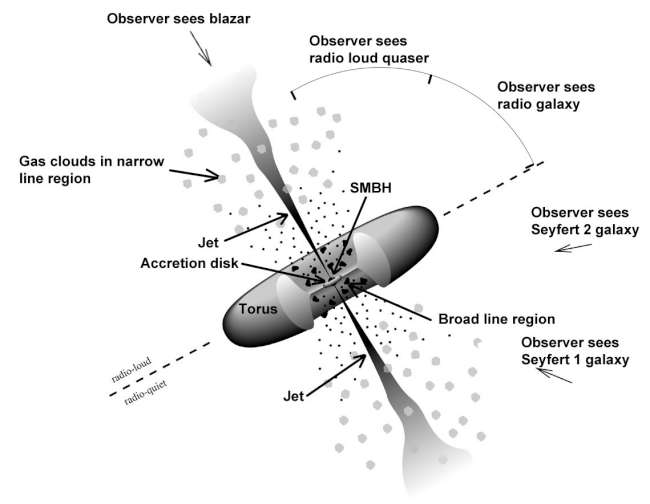
\includegraphics[width=0.7\textwidth]{Figures/AGN Structure.jpg}
    \caption{The structure of an Active Galactic Nucleus. The different regions mentioned before are labeled.}
    \label{fig:AGN_structure}
\end{figure}


\section{Radiation in AGNs}

The main topic of this project is the production of gamma rays in the AGN of NGC 1068, and how these gamma rays interact with the surrounding gas and radiation. We should first try to understand the underlying mechanisms that produce this type of radiation, as well as all the types of radiation at play in such regions.

It is also essential to make a distinction between thermal and non-thermal emission processes. Thermal emission has its origin in hot matter in the AGN. It follows a blackbody-like distribution, and is produced by particles which are in thermal equilibrium. Non-thermal emission, on the other hand, is produced by particles that are not in thermal equilibrium, and are accelerated to high energies, producing then radiation through different processes.

In general, AGNs emit radiation across the electromagnetic spectrum:

\begin{itemize}
    \item \textbf{Radio Emission:}
    \subitem \textbf{Synchrotron Radiation:} Generated by relativistic electrons spiraling in magnetic fields, which is common in AGN jets and lobes. In these sources the synchrotron spectrum typically covers photon energies from approximately $10^{-9}$ eV up to about $10^{-5}$ eV. In powerful radio-loud AGNs, this component can be extremely luminous, sometimes exceeding $10^{24}$ W Hz$^{-1}$.
    \subitem \textbf{Free-Free Emission:} Generated by the interaction of free electrons with ions in the gas, which is common in HII regions (regions of ionized hydrogen).
    \subitem \textbf{Maser Emission:} In some AGNs, molecules such as water in dense regions produce amplified microwave signals. This emission is typically observed around $10^{-6}$ eV and, while striking, generally represents only a minor fraction of the overall radio luminosity.
    
    \item \textbf{Infrared Emission:}
    \subitem \textbf{Thermal Dust Emission:} Dust in the circumnuclear torus absorbs high-energy photons and re-emits the energy in the infrared. The resulting spectrum covers energies from 0.001 to 1 eV. In obscured AGNs, this infrared component can dominate the bolometric output.
    
    \item \textbf{Optical/UV Emission:}
    \subitem \textbf{Thermal Emission:} The inner parts of the accretion disk surrounding the supermassive black hole are heated to temperatures high enough to emit thermal radiation that peaks in the optical/UV band. This emission typically spans photon energies from about 1 eV to 10 eV, and in many unobscured AGNs it is the dominant contributor to the total luminosity.
    \subitem \textbf{Broad and Narrow Line Emission:} In addition to the continuum, ionized gas in the broad-line and narrow-line regions produces characteristic spectral lines in the optical/UV. For example, the H$_{\alpha}$ line at 6563 \AA\ (about 1.89 eV) is prominent.
    
    \item \textbf{X-ray Emission:}
    \subitem \textbf{Non-thermal Emission:} Relativistic electrons in the jets can upscatter soft photons via inverse Compton scattering, producing X-rays typically in the range from 0.1 keV to 100 keV.
    
    \subitem \textbf{Bremsstrahlung:} In certain AGNs, collisions in the hot gas produce thermal X-ray emission, which generally occurs over a similar energy interval (roughly 0.1 - 100 keV). Although significant, this process usually contributes less to the total X-ray luminosity than the non-thermal component.
    
    \item \textbf{Gamma-ray Emission:}
    \subitem \textbf{Inverse Compton Scattering:} In the AGN jets, high-energy electrons collide with low-energy background photons, boosting them to gamma-ray energies. This mechanism typically yields gamma rays in the range of 100 keV up to more than 10 GeV, and in some blazars, it forms a major part of the high-energy emission.
    \subitem \textbf{Proton-Proton Interactions:} High-energy protons interacting with ambient protons can produce pions that decay into gamma rays (and neutrinos), often extending the spectrum into the TeV range (above $10^{12}$ eV). 
    \subitem \textbf{Proton-Photon Interactions:} Similarly, interactions between high-energy protons and low-energy photons lead to pion production and subsequent gamma-ray emission, further extending the high-energy tail into the TeV regime.
\end{itemize}


All in all, we get a complex distribution of energies in the AGN, with different processes producing different kinds of radiation. We can show this distribution in a spectral energy distribution (SED) plot, which shows the luminosity of the AGN as a function of frequency. Figure \ref{fig:AGN_SED} shows a schematic representation of the expected SED of a general AGN (excluding the radio and microwave bands, which are not shown).

\begin{figure}[h]
    \centering
    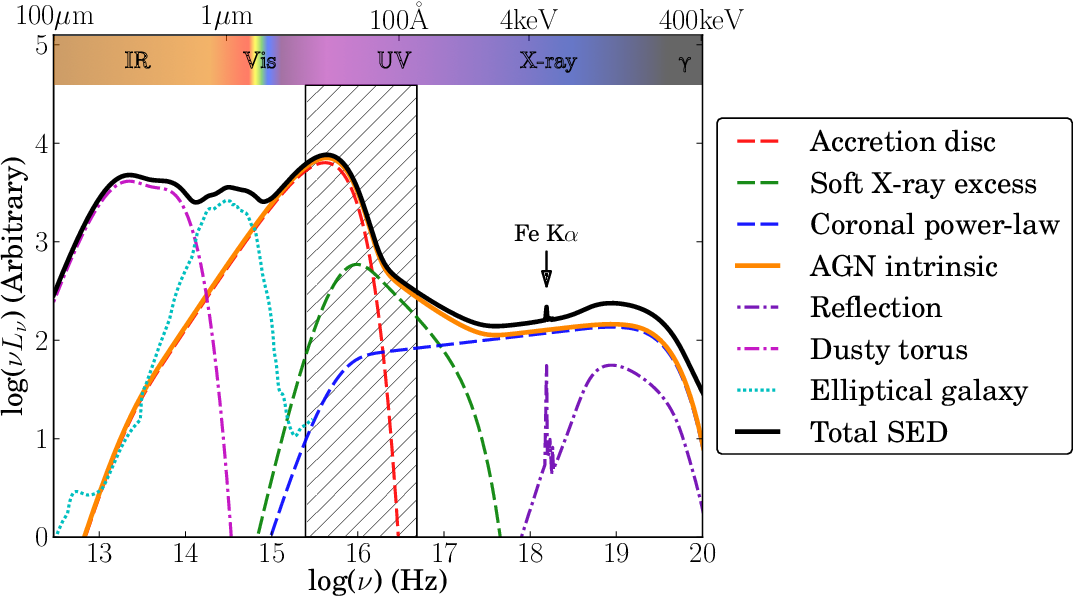
\includegraphics[width=\textwidth]{Figures/AGN SED.png}
    \caption{A simplified schematic diagram of an AGN SED, showing the approximate shape and extent of the various components discussed in the text. Dashed lines denote AGN intrinsic emission, dash-dot lines show emission reprocessed by the surrounding material and the dotted line shows starlight from an elliptical host galaxy. The hatched region highlights the spectral range that is heavily obscured by absorption in the IGM. We only show an elliptical galaxy here; galaxies with active star formation have stronger UV/IR contributions. Figure taken from \citet{QuasarSEDCollinson_2016}.}
    \label{fig:AGN_SED}
\end{figure}

Proton-proton interactions and proton-photon interactions in the AGN of NGC 1068 are of special interest, since these processes also produce neutrinos, whose energy spectrum is related to the gamma-ray spectrum in a clear and predictable manner.


\section{Gamma-ray Production in AGNs}

As mentioned above, gamma rays in AGNs are produced through different processes. We will focus on proton-proton and proton-photon interactions, which are sources of gamma rays and neutrinos in AGNs.

Inside AGNs, close to the supermassive black hole, we have a region of hot, ionized gas. This gas is composed of protons and electrons, which are accelerated to high energies by extremely high magnetic fields present in the region. These protons can then collide with other protons or photons in the gas, producing pions through the simplified processes specified below:


\begin{figure}[H]
    \centering
    \feynmandiagram [large, horizontal=a to b] {
        i1 [particle=\(p\)] -- [fermion] a,
        i2 [particle=\(\gamma\)]-- [photon] a,
        a -- c [blob, label=\(\Delta(1232)\)] -- b,
        b -- [fermion] f1 [particle=\(\pi^+_{(\nicefrac{1}{3})}\text{, }\pi^0_{(\nicefrac{2}{3})}\)],
        b -- [fermion] f2 [particle=\(n_{(\nicefrac{1}{3})}\text{, }p_{(\nicefrac{2}{3})}\)],
    };
    \caption{Proton-photon interaction.}
  \end{figure}

\begin{figure}[H]
  \centering
  \feynmandiagram [ large, horizontal=a to b] {
      i1 [particle=\(p\)] -- [fermion] a,
      i2 [particle=\(p\)]-- [fermion] a,
      a -- c [blob] -- b,
      b -- [fermion] f1 [particle=\(p\)],
      b -- [fermion] f2 [particle=\(n\text{, }p\)],
      b -- [fermion] f3 [particle = \(\pi^+\text{, }\pi^0\)],
  };
  \caption{Proton-proton interaction.}

\end{figure}

With the probabilites indicated as subindices. The pions produced then decay into gamma rays and neutrinos throught the following processes:
\vspace{-0.275cm}
\begin{figure}[H]
    \centering
    \begin{subfigure}{0.45\textwidth}
        \centering
        \feynmandiagram [medium, vertical=a to t1] {
            a [particle=\(\pi^{0}\)] -- [scalar] t1 [blob] -- [anti fermion, edge label'=\(k^-\)] t2 -- [anti fermion, edge label'=\(k^+\)] t3 -- [anti fermion, edge label'=\(k^+\)] t1,
            t2 -- [photon, blue] p1 [blue, particle=\(\gamma\)],
            t3 -- [photon, blue] p2 [blue, particle=\(\gamma\)],
            p1 -- [opacity=0] p2,
        };
        \caption{Neutral pion decay.}
    \end{subfigure}
    \begin{subfigure}{0.45\textwidth}
        \centering
        % Using the layered layout
        \feynmandiagram [layered layout, horizontal=k to b] {
        p [particle=\(\pi^{+}\)] -- [anti fermion] a [particle=\(\mu^{+}\)],
        p -- [red, fermion] d [red, particle=\(\nu_{\mu}\)],
        a  -- [anti fermion] b -- [red, anti fermion] f1 [red, particle=\(\overline \nu_{\mu}\)],
            b -- [boson, edge label'=\(W^{+}\)] c,
            c -- [red, fermion] f2 [red, particle=\(\nu_{e}\)],
            c -- [anti fermion] f3 [particle=\(e^{+}\)],
            };
        \caption{Charged pion decay.}
    \end{subfigure}
  \end{figure}

As you can see highlighted in blue and red, the pions decay into gamma rays and neutrinos, respectively.
The interesting part from this is that, since these particles come from the same source, it can be stated that a flux of neutrinos from the AGN of NGC 1068 is unavoidably accompained by a $\gamma$-ray flux $F_\gamma \sim 2 \times F_\nu$.

\section{The AGN of NGC 1068}

NGC 1068 is a Seyfert galaxy located in the constellation Cetus, approximately 47 million light-years away from Earth. It is one of the closest AGNs to our galaxy, and has been the subject of numerous studies due to its unique properties.

The publishing of data from the IceCube collaboration \citep{IceCube2022} has sparked numerous studies on the gamma-ray and neutrino emission from NGC 1068. Turning our attention to the SED of NGC 1068, we can see that the gamma-ray emission is expected to be comparable to the neutrino emission, as shown in figure \ref{fig:NGC1068_SED}.
\begin{figure}[H]
    \centering
    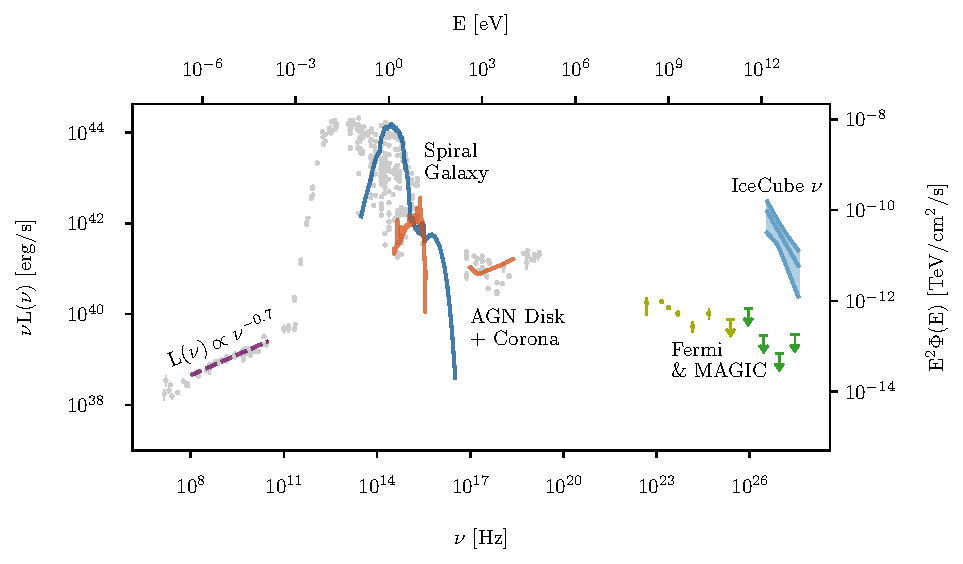
\includegraphics[width=0.7\textwidth]{Figures/NGC1068_SED.png}
    \caption{The SED of NGC 1068, showing the expected gamma-ray and neutrino emission.}
    \label{fig:NGC1068_SED}




%The background section should give sufficient background information to give the reader an overview of the state-of-the-art research field in which you work.

%The background chapter can be a bit similar to the introduction. For journal articles, it is not that common with a background section, as it is not kept separate from the introduction. However, for a master thesis, it is common to have more background and therefore to separate out some of the background material into a separate chapter. For a specialization project, the background chapter could be the most important chapter, as the specialization project is centered around learning a new subject field.

%Do not overestimate the background knowledge of the reader. As a rule of thumb, you could assume (s)he knows as much as you did when you started on your master thesis/project. So you need to give the reader enough background to be able to read the rest of your thesis.

%All relevant literature should be included, so do a thorough literature search. When you do, try not to miss out on the classics and defining papers in your field of work. For a specialization project, your background section can include references to display the breadth of the field you are working on. In contrast, for a master thesis, you should be able to argue for all included references. Do not add references just to get a long reference list. After you have spent a lot of time reading something, it could be tempting to add those references to just show off that you have read them, even though it turned out after reading them that it is not fully related to your work. Do not, all included references in your master thesis should be relevant to your work.

%The background material should also motivate your work. It should make your research question interesting by showing what others have done, and showing what is missing, highlighting the void that you try to fill with your work.


%\section{Citations}

%The background needs relevant literature to place your project work into context. The Google-scholar search (\url{scholar.google.com}) is a good starting point for searching for relevant papers.  This subsection will show how to include these references in your latex-document.

%There is a long range of different styles and packages in Latex for citations. During your writing process, it is often beneficial to have an \texttt{authoryear} style, where you see the author(s) and the year of publication. This will help you remember what the reference is. In the \texttt{main.tex} file you will find a command defining the bibliography style.

%This is where you want to go to change the style of your referencing. In this setup, we use the \texttt{natbib} style. This allows for using \verb=\citep= and \verb=\citet= references, which are useful if you use \texttt{authoryear} style:
%\begin{itemize}
 %   \item Whenever the reference is part of the sentence, you should use the textual citation \verb=\citet=. The \verb=\citet= reference types will give a reference that looks like this: \citet{berg2014permeability}.
 %   \item Whenever the reference is not a part of the sentence, but just general for the sentence or paragraph, you should use the parenthetical citation \verb=\citep=. The \verb=\citep= reference types will give a reference that looks like this: \citep{berg2014permeability}.
 %   \item If you do not specify, but use \verb=\cite=, it will look like this: \cite{berg2014permeability}.
%\end{itemize}

%All the references you use will automatically show up in your reference list. If you want to shift to numerical citations, you should use the \texttt{cite} command, as there are no differences between textual and parenthetical citations when you use the numerical style.